\title{Diagram of IsLeapYear() algorithm}
\author{
        Jonas Lindvig\\
        \hline
        jonli@itu.dk
}
\date{\today}

\documentclass[12pt]{article}
\usepackage{graphicx}


\begin{document}

\maketitle
\begin{figure}[h]
    \centering
    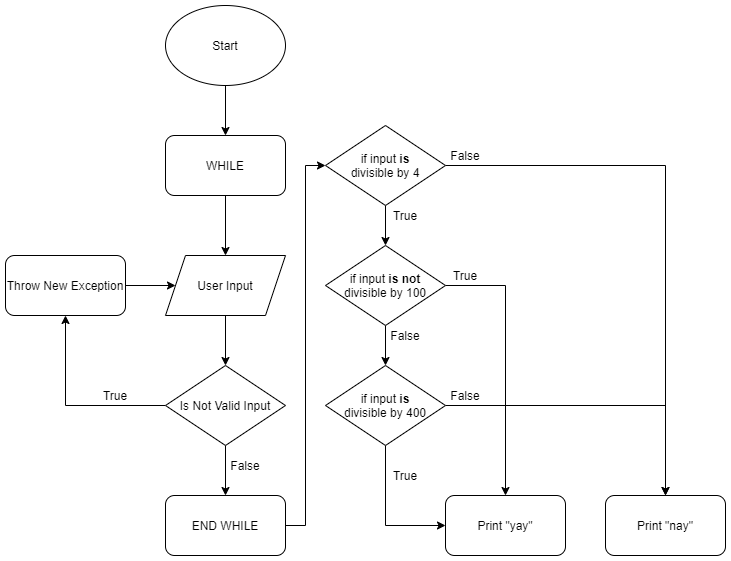
\includegraphics[width=0.8\textwidth]{images/Assignment_0_diagram.png}
    \caption{Diagram of the Main and IsLeapYear methods}
\end{figure}
The Main method enters a While-Loop in which the user is tasked with entering a year. The input throws an exception if the input can't be converted to an int, or if the year is smaller than or equal to 1582. When a valid input has been made, the IsLeapYear method checks if the year is divisible by 4, and if it either: can't be divided by 100, or can be divided by 400. If it returns true "yay" is printed, and if false is returned "nay" is printed.
\end{document}